%%%%%%%%%%%%%%%%%%%%%%%%%%%%%%%%%%%%%%%%%%%%%%%%%%%%%%%
%% Bachelor's & Master's Thesis Template             %%
%% Copyleft by Artur M. Brodzki & Piotr Woźniak      %%
%% Faculty of Electronics and Information Technology %%
%% Warsaw University of Technology, 2019-2020        %%
%%%%%%%%%%%%%%%%%%%%%%%%%%%%%%%%%%%%%%%%%%%%%%%%%%%%%%%

\documentclass[
    left=2.5cm,         % Sadly, generic margin parameter
    right=2.5cm,        % doesnt't work, as it is
    top=2.5cm,          % superseded by more specific
    bottom=3cm,         % left...bottom parameters.
    bindingoffset=6mm,  % Optional binding offset.
    nohyphenation=false % You may turn off hyphenation, if don't like.
]{eiti/eiti-thesis}

\usepackage{bm}
\langpol % Dla języka angielskiego mamy \langeng
\graphicspath{{img/}}             % Katalog z obrazkami.
\addbibresource{bibliografia.bib} % Plik .bib z bibliografią

\begin{document}

%--------------------------------------
% Strona tytułowa
%--------------------------------------
\EngineerThesis % Dla pracy inżynierskiej mamy \EngineerThesis
\instytut{Automatyki i Informatyki Stosowanej}
\kierunek{Informatyka}
\specjalnosc{Systemy Informacyjno-Decyzyjne}
\title{
	Zastosowanie algorytmów upraszczania \\ sztucznych sieci neuronowych \\
	w algorytmach regulacji
}
\engtitle{ % Tytuł po angielsku do angielskiego streszczenia
    Unnecessarily long and complicated thesis' title \\
    difficult to read, understand and pronounce
}
\author{Damian Koss}
\album{293128}
\promotor{dr inż. Patryk Chaber}
\date{\the\year}
\maketitle

%--------------------------------------
% Streszczenie po polsku
%--------------------------------------
\cleardoublepage % Zaczynamy od nieparzystej strony
\streszczenie To jest streszczenie długiej i ciężkiej pracy nie wiem 
w sumie co tutaj więcej napisać ale coś trzeba.
%\lipsum[1-3]
\slowakluczowe Sieci neuronowe, regulacja predykcyjna, upraszczanie sieci neuronowej

%--------------------------------------
% Streszczenie po angielsku
%--------------------------------------
\newpage
\abstract \kant[1-3]
\keywords XXX, XXX, XXX

%--------------------------------------
% Oświadczenie o autorstwie
%--------------------------------------
\cleardoublepage  % Zaczynamy od nieparzystej strony
\pagestyle{plain}
\makeauthorship

%--------------------------------------
% Spis treści
%--------------------------------------
\cleardoublepage % Zaczynamy od nieparzystej strony
\tableofcontents

%--------------------------------------
% Rozdziały
%--------------------------------------
\cleardoublepage % Zaczynamy od nieparzystej strony
\pagestyle{headings}

\newpage % Rozdziały zaczynamy od nowej strony.
\section{Wstęp}

\par Ciągły rozwój nauki i techniki sprawia, że wiele dziedzin życia zmienia się na naszych oczach. Obserwujemy coraz to większe dążenie do automatyzacji i informatyzacji otaczającego nas świata. Zmiany, które obserwujemy nie dotyczą jedynie przemysłu czy wąskiego grona wysoko-wyspecjalizowanych profesji ale często wkraczają już nawet do naszego życia codziennego. Komputery i roboty są  w stanie przeprowadzić za nas skomplikowaną reakcję chemiczną ale także wymieszać składniki na ciasto w odpowiednich proporcjach. 

\par Wspomniane proporcje są tutaj kluczowe stąd też z automatyzacją nieodzownie łączą się takie zagadnienia jak sterowanie i regulacja. Praktycznie każde mniej lub bardziej skomplikowane zadanie możemy zapisać w postaci konkretnego algorytmu, a następnie zrealizować go poprzez kontrolę pewnych ustalonych parametrów. Doskonałym przykładem jest tutaj dostosowanie temperatury wody w wannie lub prowadzenie samochodu. W obu tych przypadkach dążymy do osiągnięcia pewnego pożądanego rezultatu, prawidłowej temperatury wody lub odpowiedniego toru jazdy.

\par Automatyka rozwija się już od średniowiecza i w tym czasie można wyszczególnić wiele przełomowych momentów. Za jedne z głównych możemy uznać: prace J. C. Maxwella z zakresu stabilności regulacji (1863 r.), zapoczątkowanie metod częstotliwościowych analizy i syntezy układów przez H. Nyquista (1932 r.) czy w końcu zastosowanie regulacji w strukturze zamkniętej ze sprzężeniem zwrotnym poprzez opracowanie regulatora PID. Obecnie jedną z powszechnie uznanych i stosowanych metod jest regulacja predykcyjna. Jednak potrzeba automatyzacji coraz to nowych dziedzin naszego życia wymusza ciągły rozwój w obszarze automatyki i konieczność udoskonalania istniejących rozwiązań lub tworzenia zupełnie nowych. Stosowane algorytmy mogą okazać się niewystarczające gdy zadania, które przed nimi stawiamy staną się bardziej złożone i wymagać będą uwzględnienia wielu niezależnych czynników. Z pomocą mogą przyjść tutaj niewątpliwie liczne osiągnięcia w dziedzinie przetwarzania informacji, a za jedno z największych należy uznać sztuczne sieci neuronowe.

\par Rosnąca popularność i uznanie sztucznych sieci neuronowych wiąże się z ich zdolnością łatwego adaptowania się do rozwiązywania różnorodnych problemów obliczeniowych. Możliwość odwzorowania nauczonych wzorców i generalizacji nabytej wiedzy sprawia, że stały się szczytowym osiągnięciem w obszarze sztucznej inteligencji. Z tego względu oczywistym wydaje się chęć wykorzystania ich zalet i sprawdzenia zdolności adaptacyjnych także w obszarze regulacji.
  
\par Głównym celem pracy jest zastosowanie jednej z metod sztucznej inteligencji w obszarze regulacji predykcyjnej. Dzięki zastosowaniu możliwie prostych i podstawowych struktur, a za taką możemy uznać jednokierunkową sztuczną sieć neuronową, możliwe będzie przedstawienie ogólnego potencjału wykorzystania sztucznych sieci neuronowych do różnorodnych zadań stawianych przed regulatorami. Ważnym aspektem będzie także wykorzystanie algorytmu upraszczania sztucznej sieci neuronowej, który ma za zadanie poprawić możliwość generalizacji danego problemu przez sztuczną sieć neuronową. 

\par W pierwszym rozdziale pracy przybliżona zostanie literatura przedmiotu, przegląd aktualnych rozwiązań i omówienie możliwości ich uzupełnienia. Następnie zaprezentowane zostaną wszelkie założenia teoretyczne, szczegółowy opis stosowanych struktur i sposób ich wykorzystania. W kolejnym rozdziale znajdą się właściwe wyniki przeprowadzonych eksperymentów. Na końcu uzyskane rezultaty zostaną podsumowane co pozwoli na wyciągnięcie ogólnych wniosków z niniejszej pracy. 



         % Wygodnie jest trzymać każdy rozdział w osobnym pliku.
\newpage % Rozdziały zaczynamy od nowej strony.
\section{Przegląd literatury przedmiotu}
Obszerność dostępnych opracowań z zakresu automatyki jak i sztucznych sieci neuronowych sprawia, że omówienie istniejących rozwiązań zostanie podzielone na dwa etapy. Pierwszym z nich jest przegląd prac z zakresu sztucznych sieci neuronowych. Omówione zostaną zarówno pozycje teoretycznych wprowadzające w dziedzinę sztucznej inteligencji i pozwalające poczynić niezbędne założenia jak i przykłady praktycznego zastosowania wybranych struktur ze szczególnym uwzględnieniem tych, w których wykorzystane zostały algorytmy upraszczania sieci sieci neuronowych. Następnie przeanalizuję dostępną literaturę z zakresu regulacji predykcyjnej i wskaże na przykłady zastosowania sieci neuronowych w tej dziedzinie.

\par Rozpoczynając pracę nad zagadnieniem sztucznych sieci neuronowych warto zapoznać się z dwoma pozycjami \cite{haykin1999} oraz \cite{osowski2013}. Oba opracowania stanowią kompleksowy przegląd istniejących metod i mogą stanowić punkt wyjścia do każdej analizy zajmującej się tematyką sztucznych sieci neuronowych. Lektura dwóch pozycji pozwoliła mi zdecydować się na wybór jednokierunkowej sieci typu sigmoidalnego z jedną warstwą ukrytą. Jest to możliwie prosta struktura, która pozwoli zarówno na samodzielną implementację jak i będzie stanowić dobry punkt wyjścia do możliwiej dalszej analizy z wykorzystaniem bardziej skomplikowanych struktur. Moją decyzję opieram także na \cite{hornik1991} gdzie autor wykazuje, że podstawowa struktura jaką jest jednokierunkowa sieć z jedną warstwą ukrytą może stanowić uniwersalny aproksymator przy założeniu dostatecznej liczby neuronów w warstwie ukrytej oraz prawidłowego doboru funkcji aktywacji. Szczegółowe umówienie wybranej struktury przedstawione zostanie w kolejnym rozdziale pracy. 

\par Kolejnym zagadnieniem jest wybór metody redukcji sieci i jak wskazuje \cite{osowskiOBD} za jedno z lepszych rozwiązań możemy uznać metody wrażliwościowe, a w szczególności metodę Optimal Brain Damage (OBD) zaproponowaną w pracy \cite{lecun1989}. Implementacja i sprawdzenie wskazanej metody w kontekście regulacji predykcyjnej będzie ciekawym zagadnieniem i jednym z głównych celów niniejszej pracy. Możemy wskazać przykłady prac, które pozwalają nam przypuszczać, że zastosowanie OBD rzeczywiście poprawi działanie proponowanej architektury i zwiększy zdolność generalizacji. W pracy \cite{chaber2018} autorzy badają efektywność zastosowania metody OBD do redukcji rekurencyjnej sieci neuronowej z jedną warstwą ukrytą. Dzięki zastosowaniu opisywanej techniki dokumentują redukcję 60 procent wag co przyczynia się do 30-to procentowego spadku błędu popełnianego przez model. Dodatkowo warto zwrócić uwagę, że analiza została przeprowadzona na podstawie modelowania chemicznej reakcji neutralizacji, a zatem na przykładzie procesu wysoce dynamicznego. Niniejsza praca zajmować się będzie ogólnym porównaniem dwóch metod regulacji z wykorzystaniem teoretycznego obiektu, jednak mimo to osiągnięte przez autorów rezultaty możemy z pewnym przybliżeniem traktować jako punkt odniesienia w trakcie dalszej analizy.

\par Następnie warto wskazać prace porównujące różne metody redukcji sieci neuronowych, a zwłaszcza na porównanie OBD z inna metodą wrażliwością Optimal Brain Surgeon (OBS) szczegółowo opisaną w \cite{osowskiOBD}. W pracy \cite{kavzoglu1998} porównana została efektywność trzech różnych metod redukcji sieci: Magnitude Based Pruning (MP), OBD i OBS. Analizę przeprowadzono z wykorzystaniem jednokierunkowej sieci neuronowe użytej do klasyfikacji obiektów z zdjęć terenu. Przedmiot analizy jest co prawda
zupełnie odmienny jednak zbliżona architektura sieci stanowi tutaj podstawę do dokładniejszego przyjrzenia się wynikom uzyskanym przez autorów. Podobnie jak w przypadku poprzedniej pracy strukturę sieci udało zredukować się o 60 procent jednak tym razem wiązało się to jedynie z niewielką choć zauważalną poprawą klasyfikacji. Wartym zauważenia natomiast jest fakt, że OBS pozwolił na osiągnięcie najlepszych rezultatów spośród trzech metod. Co więcej nie jest to jedyna praca, w której wykazana zostaje taka zależność. Autorzy w pracy \cite{hassibi1993} porównując dwie wspomniane wcześniej metody redukcji sieci wskazują na istotny problem, a mianowicie, że OBD nie zawsze redukuje prawidłowe wagi sieci, a także w większości przypadków prowadzi do mniejszej redukcji sieci niż OBS. Analiza przeprowadzona została na podstawie przykładowego zbioru danych używanego do weryfikacji różnorodnych zagadnień uczenia maszynowego MONK's Problems Data Set. Na podstawie przedstawionych opracowań warto
rozważyć użycie nie tylko metody OBD ale poszerzenie analizy o OBS, jednak decyzja o dalszym rozwoju pracy uwarunkowana będzie jakością wyników uzyskanych za pomocą algorytmu OBD.

\par Po zapoznaniu się z pracami kluczowymi ze względu na aspekt doboru architektury sieci należy spojrzeć na przykłady zastosowania sieci neuronowych w regulacji predykcyjnej. W pracy \cite{kiti2009} autorzy badają wpływ wykorzystanie wielowarstwowej jednokierunkowej sieci neuronowej do kontroli nieliniowego wieloczynnikowego procesu chemicznego jakim jest wytrawianie metalu (Steel Pickling). Wykazane zostaje, że w przypadku procesu o podanej charakterystyce tradycyjne metody sterowania okazują się dawać gorsze rezultaty niż podejście oparte o sztuczne sieci neuronowe, które to przykładowo zdecydowanie lepiej radziły sobie z eliminacją oscylacji. 
\par Kolejnym przykładem zastosowania sieci neuronowych do regulacji procesu chemicznego jest praca \cite{hosen2011} W tym przypadku regulacja ponownie dotyczy złożonego nieliniowego procesu chemicznego, a w celu jego regulacji użyto rekurencyjnej sieci neuronowej z jedną warstwą ukrytą. Warto zauważyć tutaj fakt, że regulacja oparta o sieci neuronowe porównana zostaje z klasycznym regulatorem PID. Klasyczne podejście prowadzi do wyraźnego prze-regulowania  układu oraz zmniejsza stabilność układu. W artykule jednoznacznie wykazana zostaje wyższość metody regulacji opartej o sztuczne sieci
neuronowe jednak autorzy wskazują, że jest to głównie związane z dużą złożonością regulowanego procesu. Na tej podstawie możemy przypuszczać, że obserwować będziemy coraz więcej problemów regulacji gdzie tradycyjne metody mogą okazać się niewystarczające i szukanie rozwiązań opartych o sieci neuronowe stanie się niezbędne. 
\par Ostatnim z przykładów, który chce omówić jest praca \cite{afram2017}, w której zaprezentowano przykład wykorzystania regulacji opartej o sieci neuronowe do sterowania system inżynierii sanitarnej w budynkach mieszkalnych. Autorzy analizują wyniki uzyskane za pomocą kilku różnych architektur sieci, a jako najbardziej typowy wybór podają jednokierunkową sieć o jednej lub więcej warstwach ukrytych. Przeprowadzona analiza wskazuje, że zastosowanie regulatora opartego o sztuczne sieci neuronowe pozwoliło zredukować konsumpcję energii w zakresie nawet do 50\% w zależności od analizowanego przypadku.

\par Wyniki wszystkich trzech prac jednoznacznie wskazują na korzyści wynikające z zastosowania sztucznych sieci neuronowych w systemach regulacji. Architektura sieci w przypadku żadnej z prac nie odpowiadała tej wybranej do mojej pracy, co więcej w żadnym z podejść nie został wykorzystany algorytm OBD lub OBS. Pokazuje to, że przeprowadzenie analizy w takim zakresie może nieść za sobą duża wartość zarówno naukową jak i poznawczą. 



\newpage % Rozdziały zaczynamy od nowej strony.
\section{Opis teoretyczny rozwiązania}
W rozdziale przedstawione zostaną wszystkie założenia teoretyczne niezbędne do pełnego zrozumienia przedmiotu pracy i późniejszej interpretacji uzyskanych rezultatów. Na początku przedstawiona zostanie idea regulacji predykcyjnej wraz z algorytmem DMC oraz obiektem regulacji, który zostanie użyty w trakcie eksperymentów. W tej części pracy przydatne były opracowania \cite{stp2009} oraz \cite{tatjewski2016}. Następnie omówię architekturę sztucznej sieci neuronowej wraz z opisem funkcji aktywacji i metodą uczenia sieci. Istotnym działem z punktu widzenia niniejszej pracy jest opis algorytmu OBD czyli metody upraszczania sieci neuronowej wykorzystanej w trakcie eksperymentów. Na końcu omówię strategię, która została wykorzystana w trakcie wykonanych eksperymentów.

\subsection{Regulacja Predykcyjna}
Regulacja predykcyjna uznawana jest za jedną z zaawansowanych technik regulacji, które to zastąpiły uprzednio powszechnie stosowane regulatory PID. Dla wielowymiarowych i skomplikowanych procesów, regulacja w oparciu o identyfikacje jednego punktu charakterystyki obiektu, jak to wygląda w regulatorze PID, może okazać się nieefektywna. Rozwiązaniem jest tutaj wykorzystanie zasady przesuwanego horyzontu i wyznaczanie w każdej chwili \(kT\), gdzie T oznacza okres próbkowania, sekwencji przyszłych wartości sygnału sterującego. Idea każdego z algorytmów regulacji predykcyjnej polega na wyznaczeniu w każdej iteracji wektora przyrostów sygnału sterującego.
\begin{equation}
\Delta U(k) \, = \, [\Delta u(k|k)\quad \Delta u(k+1|k)\quad \Delta u(k+2|k)\quad ... \quad \Delta u(k + N_u - 1|k)]^T
\end{equation}
gdzie przez \(N_u\) oznaczamy horyzont sterowania, a notacja \(\Delta u(k+p|k\) oznacza przyrost sygnału sterującego obliczony w chwili \(k\), który ma być wykorzystany do sterowania w chwili \(k+p\). W istocie jednak do sterowania wykorzystuje się tylko pierwszą wartość wyznaczanego wektora i prawo regulacji w kolejnych iteracjach przyjmuje postać
\begin{equation}
u(k) \, = \, u(k|k) \, = \, \Delta u(k|k) + u(k-1)
\end{equation}

\subsubsection{Algorytm DMC}
Główna idea algorytmu DMC (Dynamic Matrix Control), przedstawionego w \cite{dmc1979}, opiera się na wykorzystaniu modelu odpowiedzi skokowej do predykcji. Algorytm DMC identyfikuje dynamikę obiektu regulacji za pomocą dyskretnych odpowiedzi skokowych, które są reakcją wyjścia w kolejnych okresach próbkowania na jednostkowy skok sygnału sterującego. Na rysunku 3.1. przedstawiono przykładową odpowiedź skokową obiektu regulacji, który to opisany zostanie w kolejnym podrozdziale. Następnie tak wyznaczona odpowiedzi skokowa obiektu \(\{s_1,\, s_2,\, s_3,\, ...\, s_D \}\) wykorzystywana jest w algorytmie DMC do wyznaczenia najbardziej optymalnych wartości sterowania. Wielkość \(D\) oznacza horyzont dynamiki obiektu i powinna zostać dobrana eksperymentalnie do takiej wartości po której wyjście obiektu ulega stabilizacji. 
\begin{figure}[!h]
    \label{fig:Odpowiedz-skokowa}
    \centering 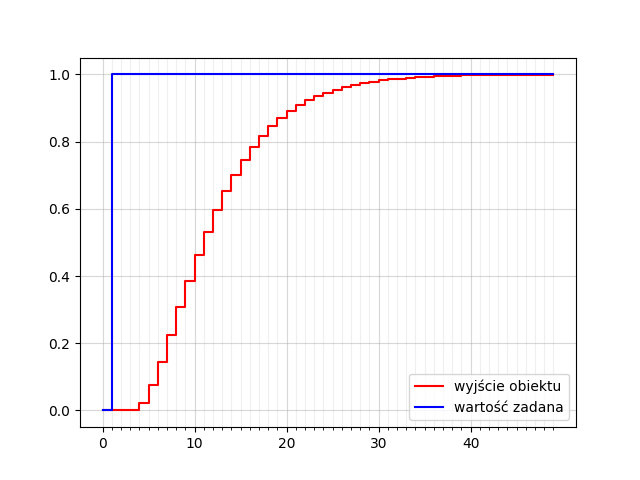
\includegraphics[width=0.7\linewidth]{Odpowiedz_skokowa.png}
    \caption{Przykładowa odpowiedź wyjścia obiektu na jednostkowy skok sterowania}
\end{figure}
\par W każdej iteracji wektor (1) wyznaczany jest w wyniku minimalizacji wskaźnika jakości, który zapisany w formie wektorowo-macierzowej przyjmuje postać
\begin{equation}
J(k) \, = \, \left\| Y^{zad}(k) - \hat{Y}(k) \right\|_{\bm{\Psi}}^2 \,+ \,\left\| \Delta U(k) \right\|_{\bm{\Lambda}}^2
\end{equation}
gdzie wektory wartości zadanej \( Y^{zad}(k) \) oraz prognozowanej trajektorii wyjścia \( \hat{Y}(k) \) o długości \( N \) będącej horyzontem predykcji definiowane są w następujący sposób
\begin{equation}
Y^{zad}(k) =
	 \begin{bmatrix}
		y^{zad}(k+1|k) \\
		\vdots \\
		y^{zad}(k+N|k)
	\end{bmatrix} , \quad
\hat{Y}(k) = 
	\begin{bmatrix}
		\hat{y}(k+1|k) \\
		\vdots \\
		\hat{y}(k+N|k)
	\end{bmatrix}
\end{equation}
macierze \( \Lambda\) oraz \( \Psi\) są macierzami diagonalnymi, a w większości przypadków przyjmują postać macierzy identyczności i takie również założenie przyjęte zostało w tej pracy. 
\par Następnie korzystając z przekształceń szczegółowo omówionych w \cite{stp2009} zapisujemy funkcję kryterialną w postaci
\begin{equation}
J(k) \, = \, \left\| Y^{zad}(k) - Y(k) - \bm{M}^P \Delta U^P(k) - \bm{M} \Delta U(k) \right\|_{\bm{\Psi}}^2 \,+ \,
\left\| \Delta U(k) \right\|_{\bm{\Lambda}}^2
\end{equation}
gdzie macierz \(M \) o wymiarowości \( N \times N_u \) ma strukturę
\begin{equation}
\bm{M} = 
	\begin{bmatrix}
		s_1 & 0 & \cdots & 0 \\
		s_2 & s_1 & \cdots & 0 \\
		\vdots & \vdots & \ddots & \vdots \\
		s_N & s_{N-1} & \cdots & s_{N-N_u+1}
	\end{bmatrix}
\end{equation}, 
macierz \(M^P \) o wymiarowości \( N \times (D-1) \) 
\begin{equation}
\bm{M^P} = 
	\begin{bmatrix}
		s_2 - s_1 & s_3 - s_2 & \cdots & s_D - s_{D-1} \\
		s_3 - s_1 & s_4 - s_2 & \cdots & s_{D+1} - S_{D-1}  \\
		\vdots & \vdots & \ddots & \vdots \\
		s_{N+1} - s_1 & s_{N+2} - s_2 & \cdots & s_{N+D-1} - s_{D-1}
	\end{bmatrix}
\end{equation}, 
natomiast wektor \( \Delta U^P(k) \) zawiera przeszłe \(D-1\) wartości zamian sygnału sterującego \(\Delta u(k-i)\). 

\par Zauważając, że funkcja jest ściśle wypukła, przyrównujemy do zera wektor gradientu funkcji i otrzymujemy wektor optymalnych przyrostów sterowania
\begin{equation}
\Delta U(k) \, = \, (\bm{M}^T\bm{\Psi}\bm{M}+\bm{\Lambda})^{-1}\bm{M}^T\bm{\Psi}(Y^{zad}(k) - Y(k) - \bm{M}^P \Delta U^P(k))
\end{equation}, 
gdzie początkową część możemy zapisać w formie 
\begin{equation}
\bm{K} \, = \, (\bm{M}^T\bm{\Psi}\bm{M}+\bm{\Lambda})^{-1}\bm{M}^T\bm{\Psi}
\end{equation}
i macierz \( \bm{K}\) jest o wymiarowości \( N_u \times N \) i wyznacza jest jednokrotnie w trakcie projektowania algorytmu. Równanie (8) jest podstawą działania algorytmu i posłuży do bezpośredniej implementacji.

\subsubsection{Obiekt regulacji}
Aby przeprowadzić niezbędne eksperymenty i dokonać porównania różnych regulatorów niezbędne jest wybranie i zaimplementowanie obiektu regulacji. W niniejszej pracy w roli obiektu wykorzystany zostanie człon inercyjny drugiego rzędu z opóźnieniem. Wybrany układ najłatwiej przedstawić w postaci równania różnicowego 
\begin{equation}
y(k) \, = \, b_1u(k-T_d-1) + b_2u(k=T_d-2)-a_1y(k-1)-a_2y(k-2)
\end{equation}
gdzie 
\begin{align*}
a_1 \, &= \, -\alpha_1 -\alpha_2 \\
a_2 \, &= \, \alpha_1\alpha_2 \\
\alpha_1 \, &= \, e^{-\frac{1}{T_1}} \\
\alpha_2 \, &= \, e^{-\frac{1}{T_2}} \\
b_1 \, &= \, \frac{K}{T_1 - T_2}[T_1(1-\alpha_1)-T_2(1-\alpha_2)] \\
b_2 \, &= \, \frac{K}{T_1 - T_2}[\alpha_1 T_2(1-\alpha_2)-\alpha_2 T_1(1-\alpha_1)]
\end{align*}

\par Dzięki takiej prezentacji i implementacji ogólnej klasy układu regulacji mamy możliwość identyfikacji poszczególnych układów poprzez cztery parametry \( T_1, \, T_2, \, K, \, T_d \). Jest to istotna własność dzięki, której w łatwy sposób można dokonywać modyfikacji obiektu i sprawdzać zachowanie regulatora w poszczególnych przypadkach.

\par Dla lepszego zrozumienia zagadnienia warto przyjrzeć się przebiegowi regulacji predykcyjnej DMC dla jednego wybranego układu regulacji. Eksperyment przedstawiony na rysunku 3.2 przeprowadzony został dla następujących parametrów \( T_1=5, \, T_2=4, \, K=1, \, T_d=3 \) i jest dla tego samego układ wcześniej pokazana została odpowiedź skokowa.  
\begin{figure}[!h]
    \label{fig:Regulacja-DMC}
    \centering 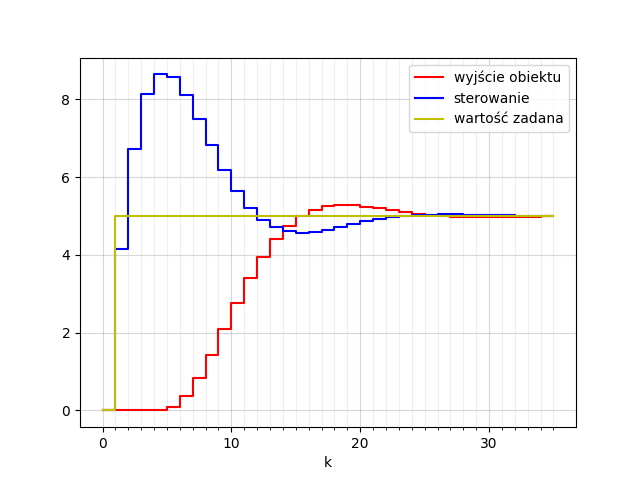
\includegraphics[width=0.7\linewidth]{Regulacja_DMC.png}
    \caption{Regulacja DMC dla wybranego obiektu}
\end{figure}
\subsection{Sztuczne Sieci Neuronowe}
Sztuczne sieci neuronowe stanowią jedną z najczęściej omawianych dziedzin przetwarzania informacji w ostatnich lat. Wielką popularność zyskały niewątpliwie dzięki swojemu interdyscyplinarnemu charakterowy, łącza one osiągnięcia biocybernetyki, elektroniki, matematyki stosowanej, statystyki oraz automatyki. Istotą działania sieci neuronowych jest próba odtworzenia zjawisk zachodzących w systemach nerwowych istot żywych poprzez zastosowanie nowoczesnych rozwiązań technologicznych.

\subsubsection{Architektura sieci}
Bazując na literaturze omówionej w poprzednim rozdziale w niniejszej pracy wykorzystana zostanie jednokierunkowa sieć typu sigmoidalnego o jednej warstwie ukrytej. Jest to jedna z najprostszych możliwych struktur, w której występują trzy warstwy neuronów wejściowa, ukryta i wyjściowa. Liczba neuronów w warstwie wejściowej i wyjściowej ściśle zależy od wymiarowości danych, natomiast największy wpływ na efektywność działania sieci ma właściwy dobór liczby neuronów w warstwie ukrytej. Poglądowy schemat jednokierunkowej sieci neuronowej przedstawiony został na rysunku 3.3. Na schemacie pokazano dwie warstwy ukryte dla lepszego zrozumienia połączeń między kolejnymi warstwami. W wyjściowej strukturze pojedynczy neuron danej warstwy połączony jest ze wszystkimi neuronami kolejnej warstwy. Liczba połączeń może być później redukowana z wykorzystywaniem algorytmu OBD, który opisany zostanie w dalszej części. 
%struktura sieci
\begin{figure}[!h]
    \label{fig:struktura-sieci}
    \centering 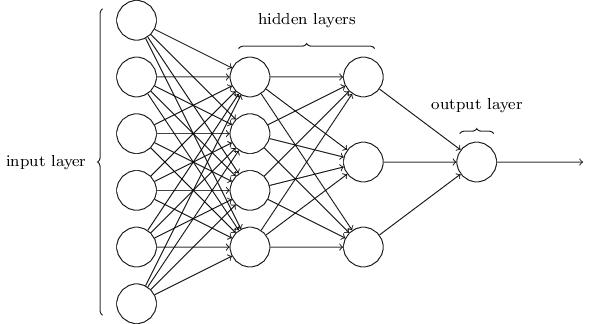
\includegraphics[width=0.7\linewidth]{struktura_sieci1.png}
    \caption{Schemat poglądowy struktury sieci. Źródło: }
\end{figure}

\par Kluczowym dla zrozumienia działania całej sieci neuronowej są przekształcenia w obrębie pojedynczego neuronu. Model neuronu przedstawiony został na rysunku 3.4. Wejścia do danego neuronu zostają przemnożone przez odpowiednie wagi, a następnie zsumowane. Następnie obliczoną sumę wykorzystujemy jako argument funkcji aktywacji przez co otrzymujemy wyjście z danego neuronu. Jedną z najczęściej stosowanych funkcji aktywacji jest funkcja sigmoidalna unipolarna o postaci 
\begin{equation}
f(z) \, = \, \frac{1}{1+e^{-z}} 
\end{equation}
, której przebieg widzimy na rysunku 3.5. Warto zauważyć, że w obrębie dostatecznie małych i dużych wartości wejścia do funkcji sigmoidalnej następuje jej stabilizacja, a co za tym idzie tak zwana stabilizacja całego neuronu.
%model neuronu
\begin{figure}[!h]
    \label{fig:struktura-sieci}
    \centering 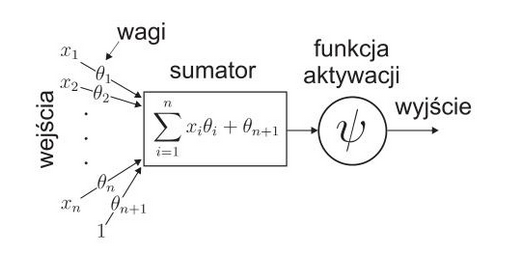
\includegraphics[width=0.6\linewidth]{model_neuronu.png}
    \caption{Model neuronu. Źródło: }
\end{figure}
%funkcja aktywacji
\begin{figure}[!h]
    \label{fig:sigmoid}
    \centering 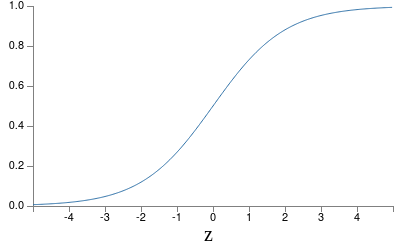
\includegraphics[width=0.5\linewidth]{sigmoid.png}
    \caption{Przebieg funkcji sigmoidalnej unipolarnej. Źródło: }
\end{figure}
\subsubsection{Wsteczna propagacja gradientu}
Uczenie sieci neuronowej możemy opisać w postaci następującego problemu. Mamy dany zbiór przykładów uczących sieci postaci \(<x,y^d> \), wektor wyjść sieci \(\bar{f}(x;\theta)\) oraz pewną funkcje straty mierzącą rozbieżność między \(y^d \) a wektorem wyjść obliczonym przez sieć, która w naszym przypadku przyjmuje postać funkcji kwadratowej, 
\begin{equation}
q(\bar{f}(x;\theta)) \, = \, \left\| \bar{f}(x;\theta) - y^d \right\|^2. 
\end{equation}
Zadaniem algorytmu uczenia jest tak dobrać wartości parametrów \( \theta \) czyli kolejnych wag sieci, aby osiągnąć minimum funkcji straty. W praktyce opiera się to na wyznaczeniu gradientu funkcji kosztu po danych parametrach, czyli wektora
\begin{equation}
\frac{dq(\bar{f}(x;\theta))}{d\theta^T}. 
\end{equation}
W praktyce wyprowadzenie konkretnych formuł na gradient funkcji za pomocą funkcji wejścia i wag może być zbyt skomplikowane. Aby uniknąć tej niedogodności stosuje się metodę wstecznej propagacji. Celem tej metody jest obliczenie pochodnych cząstkowych \( \frac{\partial q}{\partial w_{jk}^l} \) oraz \( \frac{\partial q}{\partial b_j^l} \), gdzie \( w_{jk}^l \) oznaczą wagę łączącą k-ty neuron warstwy l-1 z j-tym neuronem warstwy l, natomiast \(b_{j}^l\) oznacza wyraz wolny j-tego neuronu warstwy l. Dla łatwiejszej prezentacji algorytmu wprowadzamy wartość \( \delta_j^l \, = \, \frac{\partial q}{\partial z_j^l} \), którą możemy interpretować jako błąd j-tego neuronu l-tej warstwy czyli pochodną cząstkową po wartości zwracanej przez sumator z rysunku 3.4. 

\par Teraz możemy przedstawić algorytm wstecznej propagacji za pomocą czterech równań. Pierwszym z nich jest wyrażenie na wartości \(\delta_j^l \) dla warstwy wyjściowej \( L \) o postaci 
\begin{equation}
\delta_j^L \, = \, \frac{\partial q}{\partial a_j^L}f^{\prime}(z_j^L),
\end{equation}
które dla kwadratowej funkcji kosztu w wersji macierzowej zapisujemy jako
\begin{equation}
\delta_j^L \, = \, (a^L - y^d)\odot f^{\prime}(z_j^L),
\end{equation}
gdzie symbol \( \odot \) oznacza iloczyn Hadamarda, \( f \) jest zdefiniowaną wcześniej funkcją aktywacji, natomiast \( a_j^L = f(z_j^l) \). 
Drugim równaniem jest wyrażenie błędów neuronów l-tej warstwy poprzez wartości błędów l+1-tej warstwy. Zapis macierzowy wygląda następująco 
\begin{equation}
\delta^l \, = \, ((w^{l+1})^T\delta^{l+1}) \odot f^{\prime}(z^l). 
\end{equation}
Za pomocą równań (15) i (16) możemy wyznaczyć wektory \( \delta_j^l \) dla każdej warstwy. Dwa kolejne równania opisują powiązanie kolejnych pochodnych cząstkowych funkcji kosztu z wyznaczonymi za pomocą dwóch pierwszych równań wektorami. Kolejno dla wyrazów wolnych
\begin{equation}
\frac{\partial q}{\partial b_j^l} \, = \, \delta_j^l , 
\end{equation}
oraz wag przypisanych do poszczególnych połączeń
\begin{equation}
\frac{\partial q}{\partial w_{jk}^l} \, = \, a_k^{l-1}\delta _j^l
\end{equation}
\par Równanie 15 - 18 stanowią podstawę do dalszej implementacji. Wyprowadzenie tych równań zostało pominięte w pracy, z uwagi że algorytm wstecznej propagacji nie jest głównym aspektem niniejszej pracy, jednak uważny czytelnik może znaleźć pełny opis w pozycjach \cite{osowski2013} oraz \cite{nielsen2015}. 

\subsubsection{Algorytm OBD}
Dzięki opisanej wcześniej metodzie uczenia sieci neuronowej mamy możliwość minimalizacji błędu popełnianego przez sieć na danych uczących i weryfikujących. Niestety nie daje to pewności, że ostateczny dobór parametrów jest optymalny ze względu na wrażliwość trenowanej sieci na początkowy dobór parametrów uczenia oraz poszczególnych wartości wag. Zgodnie z \cite{osowski2013} rozwiązaniem może być tutaj zastosowanie metod redukcji sieci, a za jedną z lepszych możemy uznać algorytm OBD (Optimal Brain Damage) zaproponowany przez LeCun \cite{lecun1989}. Wskazany algorytm należy do klasy wrażliwościowych metod redukcji sieci i jego podstawowym zadaniem jest zmniejszenie liczby powiązań między-neuronowych a co za tym idzie uproszczenie struktury sieci. 
\par Idea algorytmu OBD polega na przypisaniu każdej z wag miary, która określi wrażliwość sieci na zmianę tej konkretnej wagi. Następnie wagi o najmniejszej wrażliwości mogą zostać usunięte co nie powinno wpłynąć w istotny sposób na działanie sieci, a za to pozwoli na uproszczenie jej struktury. Twórca algorytmu za miarę ważności danej wagi proponuje współczynnik asymetrii (ang. saliency), który zdefiniowany zostaje w następujący sposób
\begin{equation}
S_i \, = \, \frac{1}{2} \frac{\partial^2q}{\partial \theta_i^2} * \theta_i^2 .
\end{equation} 
Podstawą do zdefiniowania miary było rozwinięcie funkcji celu \(q\) w szereg Taylora i na tej podstawie znalezienie parametrów, których usunięcie będzie miało najmniejszy wpływ na  \(q\). Wyznaczenie pełnej macierzy Hessego \(H\) w większości przypadków staje się niemożliwie ze względu na złożoność obliczeniową. Z tego powodu LeCun wykorzystał fakt, że wobec dodatniej określoności hesjanu macierz \(H\) jest diagonalnie dominująca. Zasadnym jest zatem uwzględnienie jedynie składników diagonalnych \( h_{ii} \), które to możemy wyznaczyć dostosowując metodę wstecznej propagacji poprzednie stosowaną do pierwszych pochodnych. 
\par Podtrzymując poprzednie założenia o kwadratowej funkcji kosztu dla każdego przykładu uczącego wyliczamy miarę
\begin{equation}
h_{ii} \, = \, \frac{\partial^2q}{\partial (w_{jk}^l)^2}, 
\end{equation}  
gdzie \( w_{jk} \) jest połączeniem pomiędzy neuronami zdefiniowanym przy prezentacji algorytmu wstecznej propagacji.
Formułę możemy rozwinąć do postaci 
\begin{equation}
\frac{\partial^2 q}{\partial (w_{jk}^l)^2} \, = \, \frac{\partial^2 q}{\partial (z_j^{l})^2}(a_k^{l-1})^2 , 
\end{equation}
i zastosować wsteczną propagację w postaci
\begin{equation}
\frac{\partial^2q}{\partial (z_k^{l})^2} \, = \, f^{\prime}(z_k^l)^2 \sum_j (w_{jk}^{l+1})^2 \frac{\partial^2 q}{\partial (z_j^{l+1})^2} + f^{\prime \prime}(z_k^l) \frac{\partial q}{\partial a_k^l}. 
\end{equation}
Dodatkowo poprzez zastosowanie aproksymacji Levenberga-Marquardta możemy uprościć wzór do postaci
\begin{equation}
\frac{\partial^2q}{\partial (z_k^{l})^2} \, = \, f^{\prime}(z_k^l)^2 \sum_j (w_{jk}^{l+1})^2 \frac{\partial^2 q}{\partial (z_j^{l+1})^2}
\end{equation}
co dodatkowo daje gwarancję, że wyznaczane aproksymacje drugich pochodnych nie będą ujemne.
Dla zastosowania powyższego wzoru niezbędne jest wyznaczenie wartości granicznej czyli drugich pochodnych dla ostatniej warstwy sieci neuronowej. Stosując wspomnianą wcześniej aproksymację otrzymujemy wzór postaci
\begin{equation}
\frac{\partial^2q}{\partial (z_k^{L})^2} \, = \, 2f^{\prime}(z_k^{L})^2
\end{equation}
\par Po wyznaczeniu wartości diagonalnych \( h_{ii} \) należy uśrednić je po wszystkich przykładach uczących i na tej podstawie zgodnie ze wzorem (19) wyznaczyć współczynniki asymetrii, zgodnie z którymi przycinane będą kolejne wagi sieci. Ogólną procedurę algorytmu OBD zapisać możemy w następujących krokach: 
\begin{enumerate}
 \item Wybór właściwej architektury sieci
 \item Pełne wytrenowanie danej struktury przy użyciu jednej z metod uczenia, na przykład wstecznej propagacji
 \item Obliczenie wartości diagonalnych macierzy Hessego czyli współczynników \( h_{ii} \) 
 \item Wyznaczenie współczynników asymetrii \( S_i \)
 \item Posortowanie parametrów rosnąco według współczynników \( S_i \)
 \item Usunięcie najmniej znaczących wag
 \item Powtórzenie procedury od punktu 2, aż do osiągnięcia pożądanego kryterium wyjścia  na danych weryfikujących
\end{enumerate}
Warto zauważyć, że usunięcie wagi odbywa się poprzez ustawienie jej wartości na zero i przypisanie odpowiedniej maski, która uniemożliwia metodzie wstecznej propagacji ponowną modyfikację parametru.  

\subsection{Strategia eksperymentów}
Opisane założenia teoretyczne stanowią podstawę do implementacji rozwiązania i przeprowadzenia eksperymentów praktycznych, których wyniki przedstawione zostaną w kolejnym rozdziale. Przed przystąpieniem do prezentacji wyników warto jednak jeszcze opisać schemat według, którego zostaną one przeprowadzone. Pozwoli to czytelnikowi na ewentualną samodzielną interpretację wyników i będzie prowadziło do lepszego zrozumienia wniosków płynących z pracy. Poniższy schemat stanowi jedynie zwięzły opis strategi, a wszystkie szczegóły opisane zostaną we właściwym rozdziale. 
\par Pierwszym etap jest wygenerowanie danych, które następnie stanowić będą przykłady uczące i weryfikujące zarówno dla algorytmu wstecznej propagacji jak i OBD. Generacja danych polega na przeprowadzeniu symulacji z wykorzystaniem regulatora DMC i zdefiniowanego obiektu regulacji. Warto zwrócić uwagę na fakt, że dane uczące i weryfikujące generowane będą oddzielnie, dzięki czemu działanie sieci neuronowej weryfikowane będzie z wykorzystaniem przykładów symulacji niewystępujących w danych uczących. Jednak przed zastosowaniem otrzymanych danych w procedurze uczenia sieci niezbędne jest ich przeskalowanie do wartości z zakresu od -1 do 1. Jest to niezbędny krok wymuszony przez rodzaj zastosowanej funkcji aktywacji. Wartym zauważenia jest fakt, że koniecznym było zastosowanie modułu skalującego pozwalającego na transformację danych wejściowych w dwie strony. Sieć neuronowa wykorzystana zostanie jako regulator, a zatem procedura odwrotnego skalowania jest tutaj niezbędna. 
\par Następnie należy wytrenować sieć neuronową z wykorzystaniem opisanej metody wstecznej propagacji. Z uwagi na fakt, że następnym krokiem będzie wykorzystanie algorytmu OBD do redukcji sieci, należy zastosować lekko zmodyfikowaną strategię względem klasycznego podejścia do uczenia sieci neuronowej. Algorytm OBD wymaga aby funkcja celu była w swoim minimum, a zatem konieczne jest pełne wytrenowanie sieci na danych uczących bez stosowania kryterium wyjścia na danych weryfikujących. Algorytm uczenia sieci zakończy swoje działanie gdy zmiany funkcji kosztu w kolejnych iteracjach będą dostatecznie małe. Eksperymenty powtórzone zostaną dla różnej ilości neuronów w warstwie ukrytej oraz różnych wartości współczynnika uczącego sieci. Pozwoli to na wybór najbardziej optymalnej architektury przed przystąpieniem do procedury redukcji sieci. 
\par Kolejno zastosujemy procedurę OBD dla optymalnej struktury sieci. Redukcja sieci zgodnie z opisaną wcześniej procedurą będzie kontynuowana aż zmiana funkcji kosztu na danych weryfikujących osiągnie dostatecznie mała wartość. Dzięki takiemu podejściu otrzymamy sieć neuronową, która powinna posiadać wysokie zdolności generalizacji postawionego przed nią zadania. W celu weryfikacji otrzymanego rezultatu przeprowadzona zostanie symulacja danego układu regulacji dla różnych wartości zadanych z wykorzystaniem sieci neuronowej oraz regulatora DMC. W obu przypadkach wyznaczony zostanie błąd średnio-kwadratowy i na tej podstawie możliwe będzie porównanie dwóch zastosowanych metod i weryfikacja czy sieć neuronowa jest w stanie zastąpić klasyczny regulator.
\par Ostatnim etapem prowadzonych badań będzie przetestowanie działania sieci neuronowej jako regulatora zmodyfikowanych obiektów regulacji. Wykorzystana zostanie tutaj wcześniej opisana własność łatwej zmiany obiektu regulacji poprzez dobór odpowiednich parametrów. Przeanalizowanie zostanie również działanie sieci dla bardziej skomplikowanych przebiegów regulacji, przykładowo wielokrotnego skoku wartości zadanej.
\vspace{8mm}
\par W rozdziale przedstawione zostały wszystkie niezbędne opisy i założenia teoretyczne pozwalające na pełne zrozumienie omawianego zagadnienia. Zaprezentowane wzory i struktury stanowią bezpośrednią podstawę do praktycznej implementacji rozwiązań, której najważniejsze części przedstawione zostaną w kolejnym rozdziale. Dodatkowo lektura tego rozdziału powinna umożliwić czytelnikowi samodzielną interpretację wyników i dokładne zrozumienie charakteru pracy.   
      



\newpage % Rozdziały zaczynamy od nowej strony.
\section{Opis wybranych elementów implementacji}
Rozdział poświęcony będzie najważniejszym elementom implementacji, przedstawione w nim zostaną kody źródłowe struktur, których opis teoretyczny czytelnik mógł znaleźć w poprzednim rozdziale. 
\par Prezentacje można podzielić na trzy oddzielne fragmenty, w pierwszej pokazana zostanie implementacja algorytmu DMC wraz z używanym w trakcie eksperymentów obiektem regulacji. Następnie czytelnik pozna najważniejsze elementy dotyczące implementacji sieci neuronowej ze szczególnym uwzględnieniem algorytmu OBD, któremu poświęcony jest ostatni podrozdział. Całość rozwiązania zaimplementowana została z wykorzystaniem języka Python 3.6 i korzysta z kilku podstawowych zewnętrznych bibliotek. Za kluczową ze względu na charakter pracy należy uznać bibliotekę NumPy pozwalająca na obsługę wielowymiarowych tablic i macierzy, a także udostępniającą zbiór funkcji matematycznych wysokiego poziomu do obsługi tych tablic. W trakcie implementacji nieocenione okazały się opracowania \cite{nielsen2015} oraz \cite{wawrzynski2019}. 

\subsection{Algorytm DMC z obiektem regulacji}
Algorytm regulacji predykcyjnej zaimplementowany został jako klasa DMC, której strukturę widzimy w poniższym kodzie:
\begin{listing}[!htb]
\captionof{listing}{Klasa \texttt{DMC}}
\begin{minted}{python}
class DMC(object):
 def __init__(self, n_u, n, S_list, psi_const, lambda_const):		
  #horyzont sterwania 
  self.n_u = n_u
  #horyzont predykcji
  self.n = n 
  #horyzont dynamiki obiektu - ile s wyzaczamy (10, 20, 30)
  self.d = len(S_list)
  self.Y_k = np.zeros(n)
  #wektor wartosci zadanej - stala na calym horyzoncie N
  self.Y_zad = np.zeros(n)
  #wektor opisujacy trajektorie sygnalu wyjsciowego 
  self.Y_hat = np.zeros(n)
  #wektor wyznaczanych przyrostow wartosci sterowania 
  self.U_delta = np.zeros(n_u)
  #wektor przeszlych przyrostow sterowania
  self.U_delta_P = np.zeros(len(S_list)-1)		
  #macierze wyznaczane w trakcie inicjalizacji klasy
  self.Psi = np.diag([psi_const for i in range(n)])
  self.Lambda = np.diag([lambda_const for i in range(n_u)])
  self.M_p = self.init_M_p(S_list, n)
  self.M = self.init_M(S_list, n, n_u)
  self.K = inv(self.M.T @ self.Psi @ self.M + self.Lambda) @ self.M.T @ self.Psi
\end{minted}
\end{listing}

Klasa inicjalizowana jest zgodnie z opisem teoretycznym w sekcji~3.1.1. z wykorzystaniem wektora odpowiedzi skokowej układu reprezentowanego przez argument \texttt{S{\_}list}. Warto zwrócić tutaj uwagę na linie~23 Listingu~1, która stanowi bezpośrednią implementację macierzy \(K\) przedstawionej za pomocą równania~(9).
\par W dalszej części występują funkcje pomocnicze wykorzystywane do tworzenia macierzy \(M\) oraz \(M^P\), których implementacja przedstawiona została na Listingu~2.

\begin{listing}[!htb]
\captionof{listing}{Funkcje wyznaczające macierze \(M\) oraz \(M^P\)}
\begin{minted}{python}
def init_M_p(self, S_list, N):
 arr=np.zeros((N,len(S_list)-1))
 for i in range(N):
  for j in range(len(S_list)-1):
   arr[i][j] = (S_list[i+j+1] if i+j+1+1<=len(S_list) else S_list[-1]) - S_list[j]
 return arr

def init_M(self, S_list, n, n_u):
 arr=np.zeros((n,n_u))
 for i in range(n):
  for j in range(i+1 if i+1<=n_u else n_u):
   arr[i][j]= S_list[i-j] if i-j+1<=len(S_list) else S_list[-1]
 return arr
\end{minted}
\end{listing}

Kluczowym elementem całej klasy ze względu na działanie algorytmu jest funkcja wyznaczająca wektor optymalnych przyrostów sterowania w każdej iteracji algorytmu. Implementację funkcji prezentuje Listing~3, gdzie w linii~3 zaimplementowano równanie~(8). W każdej iteracji algorytmu zwracana jest tylko wartość \(\Delta u(k|k) \), której odpowiada zwracana przez funkcję zmienna \texttt{delta{\_}u}.

\begin{listing}[!htb]
\captionof{listing}{Funcja wyznaczająca wektor przyrostów sterowania}
\begin{minted}{python}
def calculate_U_delta(self, Y_current): 
 self.Y_k.fill(Y_current)
 self.U_delta = self.K @ (self.Y_zad - self.Y_k - (self.M_p @ self.U_delta_P))
 delta_u = self.U_delta[0]
 self.update_U_delta_P(delta_u)
 return delta_u
\end{minted}
\end{listing}

\par Obiekt regulacji zaimplementowany został w postaci klasy \texttt{SimObject} gdzie istotę działania obiektu prezentuje funkcja zwracająca wyjście obiektu na podstawie wartości sterowania, w każdej kolejnej iteracji. Listing~4 prezentuje funkcję   \texttt{make{\_}simulation{\_}step}, w której należy zwrócić uwagę na linie 6, w której widzimy zaimplementowane równanie~(10).

\begin{listing}[!htb]
\captionof{listing}{Funkcja zwracająca wyjście obiektu sterowania}
\begin{minted}{python}
def make_simulation_step(self, u, y_zad):		
 u_lag1=self.get_lag_u(self.TD+1)
 u_lag2=self.get_lag_u(self.TD+2)
 y_lag1=self.get_lag_y(1)
 y_lag2=self.get_lag_y(2)
 y_current=self.b_1*u_lag1 + self.b_2*u_lag2 - self.a_1*y_lag1 - self.a_2*y_lag2
 self.y_list = np.append(self.y_list, y_current)
 self.u_list = np.append(self.u_list, u)
 self.y_zad_list = np.append(self.y_zad_list, y_zad)
 return y_current
\end{minted}
\end{listing}
 
\subsection{Architektura sieci neuronowej}
Implementacja sieci neuronowej przedstawiona została w postaci klasy \emph{Network}, której konstruktor widzimy w Listingu~5. Struktura sieci składa się z listy macierzy \texttt{weights} (linia~6) oraz \texttt{biases} (linia~5) odpowiadających kolejnym wagom oraz wyrazom wolnym dla połączeń między neuronami sąsiadujących warstw. Natomiast lista macierzy \texttt{saliencies} o tej samej wymiarowości co \texttt{weights} zawierają współczynniki asymetrii wyznaczane w trakcie działania algorytmu OBD. Zmienna \texttt{mask} wykorzystywana jest przez algorytm OBD do zamrożenia danych wag w trakcie ponownego uczenia sieci. Na końcu inicjalizacji ustalany jest parametr \texttt{cost{\_}delta{\_}epsilon} stanowiący graniczną wartość gradientu funkcji celu poniżej, której proces uczenia sieci zostaje zakończony. 
  
\begin{listing}[!htb]
\captionof{listing}{Klasa \texttt{Network}}
\begin{minted}{python}
class Network(object):
 def __init__(self, sizes): 
  self.num_layers = len(sizes)
  self.sizes = sizes
  self.biases = [np.random.randn(y, 1) for y in sizes[1:]]
  self.weights = [np.random.randn(y, x) for x, y in zip(sizes[:-1], sizes[1:])]
  self.saliencies = [np.zeros((y, x)) for x, y in zip(sizes[:-1], sizes[1:])]
  self.mask = [np.ones((y, x)) for x, y in zip(sizes[:-1], sizes[1:])]
  self.cost_delta_epsilon = 0.000005
\end{minted}
\end{listing}

\par Główną część implementacji sieci neuronowej stanowią funkcje wykorzystywane w trakcie procesu trenowania sieci. Jest to odpowiednio funkcja \texttt{SGD} implementująca metodę stochastycznego najszybszego spadku SGD \emph{(Stochastic Gradient Descent)}, jedną z najczęściej stosowanych metod iteracyjnej optymalizacji funkcji celu. Metoda to korzysta z funkcji \texttt{update{\_}mini{\_}batch}, która to odpowiada za zastosowanie metody wstecznej propagacji dla każdego z przykładów uczących występujących w pojedynczej próbce wyznaczanej przez SGD. Kluczowym dla działania wymienionych funkcji jest implementacja metody wstecznej propagacji dla pojedynczego przykładu uczącego. Teoretyczne założenia używanej metody przedstawione zostały w sekcji 3.2.2, a jej implementację widzimy na Listingu~6. W początkowej części (linie~2-3) tworzone są wektory odpowiadające pochodnych cząstkowych \( \frac{\partial q}{\partial w_{jk}^l} \) oraz \( \frac{\partial q}{\partial b_j^l} \). Następnie w liniach~5-12 następuje jednokrotne przejście sieci w przód (\emph{ang. feedforward}) czyli wyliczenie wyjścia sieci na podstawie wektora wejściowego \emph{x}. Główna zasada działania wstecznej propagacji znajduje odzwierciedlenie w kolejnych liniach kodu. Należy zwrócić tutaj szczególną uwagę na linie~15, gdzie wykorzystane zostało równanie~(15) stanowiące warunek początkowy dla algorytmu. Następnie w pętli następuje wsteczna propagacja między warstwami opisana równaniem~(16), które znajduje bezpośrednie odzwierciedlenie w linii~22.

\begin{listing}[!htb]
\captionof{listing}{Funkcja wstecznej propagacji}
\begin{minted}{python}
def backprop(self, x, y):
 nabla_b = [np.zeros(b.shape) for b in self.biases]
 nabla_w = [np.zeros(w.shape) for w in self.weights]
 # jednokrotne wyznaczenie wyjscia sieci dla wjescia x
 activation = x
 activations = [x] 
 zs = []
 for b, w in zip(self.biases, self.weights):
   z = np.dot(w, activation)+b
   zs.append(z)
   activation = sigmoid(z)
   activations.append(activation)
 # wsteczna propagacja
 # warunek poczatkowy
 delta = self.cost_derivative(activations[-1], y) * sigmoid_prime(zs[-1])
 nabla_b[-1] = delta
 nabla_w[-1] = np.dot(delta, activations[-2].transpose())
 # iteracja od konca po warstwach
 for l in range(2, self.num_layers):
   z = zs[-l]
   sp = sigmoid_prime(z)
   delta = np.dot(self.weights[-l+1].transpose(), delta) * sp
   nabla_b[-l] = delta
   nabla_w[-l] = np.dot(delta, activations[-l-1].transpose())
 return (nabla_b, nabla_w)
\end{minted}
\end{listing}

\par Pozostała część implementacji obejmuje funkcje aktywacji, funkcje wyliczającą wyjście sieci na podstawie zadanego wektora wejściowego, a także wszelkie niezbędne funkcje pomocnicze. Sposób ich implementacji nie jest kluczowy dla zrozumienia całości pracy, a może być w łatwy sposób odtworzony na podstawie opisu teoretycznego. Z punktu widzenia czytelnika warto jednak przyjrzeć się ostatniej części klasy \texttt{Network}, która zawiera implementację algorytmu redukcji sieci OBD.

\subsection{Algorytm OBD}
Algorytm OBD zaimplementowany został jako część klasy \texttt{Network} na podstawie opisu teoretycznego zawartego w sekcji 3.2.3. i składa się z trzech głównych funkcji \texttt{OBD}, \texttt{backpropOBD} oraz \texttt{cut{\_}weights}. Pierwsza z nich przedstawiona została na Listingu~7 i odpowiada za implementację procedury algorytmu OBD  przedstawionej w opisie teoretycznym. Kluczowa dla działania algorytmu jest pętla rozpoczynająca się w linii 8, która kolejno wywołuje metodę wstecznej propagacji dla drugich pochodnych. Po iteracji dla wszystkich przykładów uczących obliczana jest wartość współczynników asymetrii i następnie w linii~15 wywoływana jest funkcja \texttt{cut{\_}weights} odpowiedzialna za przycinanie sieci. Po redukcji sieć jest ponownie uczona z wykorzystaniem metody \texttt{SGD}. Procedura zostaje powtórzona aż do osiągnięcia kryterium wyjścia na danych testujących.
\begin{listing}[!htb]
\captionof{listing}{Algorytm OBD}
\begin{minted}{python}
def OBD(self, train_data, test_data):
 nabla_h = [np.zeros(w.shape) for w in self.weights]
 par_number = sum([w.shape[0]*w.shape[1] for w in self.weights])
 test_cost = []
 prev_cost = np.inf
 prev_delta_cost_list = np.full((3,),np.inf)

 for limit in range(int(0.9*par_number)):
   for x, y in train_data:
     delta_nabla_h = self.backpropOBD(x,y)
     nabla_h = [nh + dnh
       for nh, dnh in zip(nabla_h, delta_nabla_h)]

   self.saliencies = [(h * w**2)/(2 * len(train_data)) for w, h in zip(self.weights, nabla_h)]
   self.cut_weights(limit+1)
   self.SGD(train_data, 200, 10, 3.0)        
   test_cost.append(self.total_cost(test_data))    
   current_cost = self.total_cost(test_data)            
   prev_delta_cost_list = np.delete(np.insert(prev_delta_cost_list, 0, prev_cost - current_cost),-1)
   prev_cost = current_cost
   #stopping rule
   if all(prev_delta_cost_list < self.cost_delta_epsilon/100):
     return train_cost, test_cost 

 return train_cost, test_cost
\end{minted}
\end{listing}

\par Niezbędnym dla zrozumienia całego algorytmu OBD jest proces wstecznej propagacji zastosowany dla drugich pochodnych. Jego implementacja zaprezentowana została na Listingu~8 i zawiera wiele podobieństw do wcześniej omawianej funkcji \texttt{backprop}. Należy zwrócić tutaj szczególną uwagę na linie~21, która odpowiada równaniu~(23). W linii~14 widzimy natomiast wykorzystanie funkcji pomocniczej do wyliczenia warunku granicznego z równania~(24), zabieg ten sprzyja czytelności kodu, a z uwagi na mało skomplikowaną formę równania nie powinien stanowić utrudnienia w zrozumieniu całej metody.
\begin{listing}[!htb]
\captionof{listing}{Funkcja wstecznej propagacji drugich pochodnych}
\begin{minted}{python}
def backpropOBD(self, x, y):       
 h_vector = [np.zeros(w.shape) for w in self.weights]
 # feedforward
 activation = x
 activations = [x] 
 zs = []
 for b, w in zip(self.biases, self.weights):
   z = np.dot(w, activation)+b
   zs.append(z)
   activation = sigmoid(z)
   activations.append(activation)
   
 #wsteczna propagacja drugich pochodnych
 delta2_z = self.boundry_OBD_derivative(zs[-1], y)
 h_vector[-1] = np.dot(delta2_z, activations[-2].transpose()**2)
 #iteracja po kolejnych warstwach
 for l in range(2, self.num_layers):
   z = zs[-l]
   sp = sigmoid_prime(z)
   sp2 = sigmoid_second_prime(z)    
   delta2_z =  sp**2 * np.dot(self.weights[-l+1].transpose()**2, delta2_z)             
   h_vector[-l] = np.dot(delta2_z, activations[-l-1].transpose()**2)
           
 return h_vector
\end{minted}
\end{listing}

\begin{listing}[!htb]
\captionof{listing}{Funkcja redukcji wag}
\begin{minted}{python}
def cut_weights(self, limit):
 saliencies_list = []
 for i_layer , saliencies in enumerate(self.saliencies):
  for i_row, row in enumerate(saliencies.tolist()):
   for i_column, value in enumerate(row):
    saliencies_list.append(( [i_layer, i_row, i_column], value))                    
 saliencies_list.sort(key = lambda x: x[1])
 to_cut = [element[0] for element in saliencies_list[:limit]]
 
 self.restore_mask()
 for wt_index in to_cut:
  self.weights[wt_index[0]][wt_index[1]][wt_index[2]] = 0.0
  self.mask[wt_index[0]][wt_index[1]][wt_index[2]] = 0.0
\end{minted}
\end{listing}

\par Ostatnią z wykorzystywanych funkcji w procedurze OBD jest funkcja \texttt{cut{\_}weights}, która pokazana została na Listingu~9. Odpowiada ona za przycięcie odpowiedniej ilości wag, ustalanej przez parametr \texttt{limit} według posortowanych wartości współczynników skośności. W liniach~2-7 współczynniki są sortowane aby następnie w zmiennej \texttt{to{\_}cut} zapisać indeksy odpowiednich wag, które to następnie zostają przycięte i zamrożone z wykorzystaniem opisywanej wcześniej maski.
\par Lektura powyższego rozdziału stanowiąca uzupełnienie do opisu teoretycznego powinna dać czytelnikowi pełny obraz wykorzystywanych w trakcie eksperymentów struktur. Po zapoznaniu się z elementami implementacji można przejść do rozdziału opisującego wyniki przeprowadzonych eksperymentów. Warto zauważyć, że zrozumienie wszystkich przedstawionych w tym rozdziale szczegółów nie jest warunkiem koniecznym do wyciągnięcia ogólnych wniosków z kolejnego rozdziału lecz na pewno stanowi dużą wartość dodaną dla czytelnika niezaznajomionego z prezentowaną w tej pracy tematyką.
\newpage % Rozdziały zaczynamy od nowej strony.
\section{Wyniki pracy}

\subsection{Generacja danych}
\subsection{Uczenie sieci neuronowej}
\subsection{Zastosowanie algorytmu OBD}
\subsection{Weryfikacja rozwiązania}
%\newpage % Rozdziały zaczynamy od nowej strony.
\section{De Finibus Bonorum et Malorum}
\lipsum[1] Lorem ipsum dolor sit amet\footnote{Lorem ipsum dolor sit amet, consectetur adipiscing elit, sed do eiusmod tempor incididunt ut labore et dolore magna aliqua. Ut enim ad minim veniam, quis nostrud exercitation ullamco laboris nisi ut aliquip ex ea commodo consequat.}.
\begin{align*}
    E & = mc^2 \\
    y & = ax^2 + bx + c
\end{align*}

\lipsum[3]

\begin{align}
\begin{bmatrix}
    1 & 0 & 0 \\
    0 & 2 & 0 \\
    0 & 0 & 3
\end{bmatrix} \cdot
\begin{bmatrix}
    4 \\ 5 \\ 6
\end{bmatrix} =
\begin{bmatrix}
    4 \\ 10 \\ 18
\end{bmatrix}
\end{align}

\lipsum[4] Lorem ipsum dolor sit amet, consectetur adipiscing elit, sed do eiusmod tempor incididunt ut labore et dolore magna aliqua \cite{szczypiorski2015}, \cite{duqu2011}, \cite{shs2015}, \cite{wozniak2018}, \cite{dcp19}.

\subsection{Critique of Pure Reason}
\kant[1]

\begin{table}[!h] \label{tab:tabela1} \centering
\caption{Przykładowa tabela.}
\begin{tabular} {| c | c | r |} \hline
    Kolumna 1 & Kolumna 2 & Liczba \\ \hline\hline
    cell1 & cell2 & 60 \\ \hline
    cell4 & cell5 & 43 \\ \hline
    cell7 & cell8 & 20,45 \\ \hline
    \multicolumn{2}{|r|}{Suma:} & 123,45 \\ \hline
\end{tabular}
\end{table}

\kant[2]

\begin{longtable}{| c | m{0.58\linewidth} | r | m{0.1\linewidth} |}
    \caption{Tabela wielostronicowa.} \\
    \hline
    Lp & \multicolumn{1}{c|}{Treść} & \multicolumn{1}{c|}{Kwota} & \multicolumn{1}{m{0.1\linewidth}|}{Wariant opłaty} \\ \hline\hline \endfirsthead

    \endfoot
    \hline \endlastfoot

    1 & Lorem ipsum dolor sit amet, consectetur adipiscing elit, sed do eiusmod tempor incididunt ut labore et dolore magna aliqua. & 111 111,11 zł & \multicolumn{1}{c|}{WAR1} \\ \hline
    2 & Lorem ipsum dolor sit amet, consectetur adipiscing elit, sed do eiusmod tempor incididunt ut labore et dolore magna aliqua. & 22 222,22 zł & \multicolumn{1}{c|}{WAR1} \\ \hline
    3 & Lorem ipsum dolor sit amet, consectetur adipiscing elit, sed do eiusmod tempor incididunt ut labore et dolore magna aliqua. & 33 333,33 zł & \multicolumn{1}{c|}{WAR1} \\ \hline
    4 & Lorem ipsum dolor sit amet, consectetur adipiscing elit, sed do eiusmod tempor incididunt ut labore et dolore magna aliqua. & 444 444,44 zł & \multicolumn{1}{c|}{WAR1} \\ \hline
    5 & Lorem ipsum dolor sit amet, consectetur adipiscing elit, sed do eiusmod tempor incididunt ut labore et dolore magna aliqua. & 55 555,55 zł & \multicolumn{1}{c|}{WAR1} \\ \hline
    6 & Lorem ipsum dolor sit amet, consectetur adipiscing elit, sed do eiusmod tempor incididunt ut labore et dolore magna aliqua. & 66 666,66 zł & \multicolumn{1}{c|}{WAR1} \\ \hline
    7 & Lorem ipsum dolor sit amet, consectetur adipiscing elit, sed do eiusmod tempor incididunt ut labore et dolore magna aliqua. & 777 777,77 zł & \multicolumn{1}{c|}{WAR1} \\ \hline
    8 & Lorem ipsum dolor sit amet, consectetur adipiscing elit, sed do eiusmod tempor incididunt ut labore et dolore magna aliqua. & 8 888,88 zł & \multicolumn{1}{c|}{WAR1} \\ \hline
    9 & Lorem ipsum dolor sit amet, consectetur adipiscing elit, sed do eiusmod tempor incididunt ut labore et dolore magna aliqua. & 999 999,99 zł & \multicolumn{1}{c|}{WAR1} \\ \hline
    10 & Lorem ipsum dolor sit amet, consectetur adipiscing elit, sed do eiusmod tempor incididunt ut labore et dolore magna aliqua. & 111 111,11 zł & \multicolumn{1}{c|}{WAR2} \\ \hline
    11 & Lorem ipsum dolor sit amet, consectetur adipiscing elit, sed do eiusmod tempor incididunt ut labore et dolore magna aliqua. & 22 222,22 zł & \multicolumn{1}{c|}{WAR2} \\ \hline
    12 & Lorem ipsum dolor sit amet, consectetur adipiscing elit, sed do eiusmod tempor incididunt ut labore et dolore magna aliqua. & 33 333,33 zł & \multicolumn{1}{c|}{WAR2} \\ \hline
    13 & Lorem ipsum dolor sit amet, consectetur adipiscing elit, sed do eiusmod tempor incididunt ut labore et dolore magna aliqua. & 444 444,44 zł & \multicolumn{1}{c|}{WAR2} \\ \hline
    14 & Lorem ipsum dolor sit amet, consectetur adipiscing elit, sed do eiusmod tempor incididunt ut labore et dolore magna aliqua. & 55 555,55 zł & \multicolumn{1}{c|}{WAR2} \\ \hline
    15 & Lorem ipsum dolor sit amet, consectetur adipiscing elit, sed do eiusmod tempor incididunt ut labore et dolore magna aliqua. & 66 666,66 zł & \multicolumn{1}{c|}{WAR2} \\ \hline
    & \multicolumn{1}{r|}{\textbf{Suma:}} & \textbf{7 777 777,77 zł} &
    \label{table:koszty}
\end{longtable}
\kant[4]

\subsection{Categorical Imperative}
\subsubsection{Deontological Ethics}
As any dedicated reader can clearly see, the Ideal of practical reason is a representation of, as far as I know, the things in themselves; as I have shown elsewhere, the phenomena should only be used as a canon for our understanding:
% Parametr label ustawia symbol, a leftmargin - wielkość wcięcia.
% Domyślny układ to [---] bez wcięcia, bo tak pan Marcin Woliński powiedział;
% ale ja nie polecam. // AB
\begin{itemize}
    \item Item 1:
    \begin{itemize}[label=---]
        \item item 1.1;
        \item item 1.2;
        \item item 1.3;
    \end{itemize}
    \item Item 2;
    \item Item 3;
    \item Item 4.
\end{itemize}
\kant[2]

\subsubsection{Consequentialism -- the Ideal of practical reason}
\kant[3]
\begin{enumerate}
    \item Item 1:
    \begin{enumerate}
        \item item 1.1;
        \item item 1.2:
        \begin{enumerate}
            \item item 1.2.1;
            \item item 1.2.2;
        \end{enumerate}
        \item item 1.3;
    \end{enumerate}
    \item Item 2;
    \item Item 3;
    \item Item 4.
\end{enumerate}

\kant[9]

\subsection{G\"odel's ontological proof}
\kant[9] Lorem ipsum dolor sit amet, consectetur adipiscing elit, sed do eiusmod tempor incididunt ut labore et dolore magna aliqua \cite{benzmuller2014}, \cite{goedel95}, \cite{wang97}, \cite{koons2005}.
\begin{assumption} \label{ass:1}
    $ [\![ \ \phi \ ]\!] \Longrightarrow [\![ \ P(\phi); \neg P(\phi) \ ]\!]$
\end{assumption}
\begin{axiom}[Dualność] \label{axiom:1}
    $\neg P(\phi) \Leftrightarrow P(\neg \phi)$, równoważnie $P(\phi) \Leftrightarrow \neg P(\neg \phi)$
\end{axiom}
\begin{axiom}[Całkowitość] \label{axiom:2}
    $ \left( P(\phi) \wedge \forall x: \phi(x) \Rightarrow \psi(x) \right) \Rightarrow P(\psi) $
\end{axiom}
\begin{axiom}[Absolutność] \label{axiom:3}
    $ P(\phi) \Rightarrow \Box P(\phi) $
\end{axiom}
\begin{definition} \label{def:1}
    $ G(x) \Leftrightarrow \forall \phi: \left( P(\phi) \Rightarrow \phi(x) \right) $
\end{definition}
\begin{definition} \label{def:2}
    $ \phi \ ess \ x \Leftrightarrow \phi(x) \wedge \forall \psi \left( \psi(x) \Rightarrow \Box \forall y \left( \phi(y) \Rightarrow \psi(y) \right) \right)  $
\end{definition}
\begin{axiom} \label{axiom:4}
    P(G)
\end{axiom}
\begin{lemma} \label{lemma:1}
    $ P(\phi) \Rightarrow \Diamond \exists x : \phi(x) $
\end{lemma}
\begin{proof}
    Dowód pomijamy, bo jest trywialny :)
\end{proof}
\begin{lemma} \label{lemma:2}
    $ \Diamond \exists x : G(x) $
\end{lemma}
\begin{proof}
    Natychmiastowy wniosek z aksjomatu \ref{axiom:4} i lematu \ref{lemma:1}.
\end{proof}
\begin{lemma} \label{lemma:3}
    $ G(x) \Rightarrow G \ ess \ x $
\end{lemma}
\begin{proof}
    Poprzez podstawienie do definicji \ref{def:2}.
\end{proof}
\begin{definition} \label{def:3}
    $ E(x) \Leftrightarrow \forall \phi \left( \phi \ ess \ x \Rightarrow \Box\ \exists x: \phi(x) \right) $
\end{definition}
\begin{axiom} \label{axiom:5}
    P(E)
\end{axiom}
\begin{theorem}
    $ \Box\ \exists x : G(x) $
\end{theorem}
\begin{proof}
    Na podstawie definicji \ref{def:1}, lematu \ref{lemma:3} i aksjomatu \ref{axiom:5}.
\end{proof}    % Umożliwia to również łatwą migrację do nowej wersji szablonu:
%\newpage % Rozdziały zaczynamy od nowej strony.
\section{Code listings}

\lipsum[10]

% \addmargin pozwala na wcięcie kodu od lewej (tutaj: 6mm).
% Wcięcie pomaga ustawić kod tak, 
% aby numery linii nie były za bardzo na lewo. 
% Druga liczba oznacza wcięcie od prawej. 
\begin{addmargin}[6mm]{0mm}
\begin{lstlisting}[
    language=HTML,
    numbers=left,
    firstnumber=1,
    caption={\emph{Hello world} w HTML},
    aboveskip=10pt
]
<html>
  <head>
    <title>Hello world!</title>
  </head>
  <body>
    Hello world!
  </body>
</html>
\end{lstlisting}
\end{addmargin}

\lipsum[11]

% Dla dłuższych numerów linii
% potrzebne jest większe wcięcie.
\begin{addmargin}[10mm]{0mm}
\begin{lstlisting}[
    language=C++,
    numbers=left,
    firstnumber=147,
    caption={Generowanie sekwencji Collatza w języku C++},
    aboveskip=10pt
]
class Collatz {
  private:
    unsigned current_val_;
    void update_val() {
        if( current_val_ % 2 == 0 )
            current_val_ /= 2;
        else
            current_val_ = current_val_ * 3 + 1;
    }

  public:
    explicit Collatz(unsigned initial_value) : 
        current_val_(initial_value) {}
    void print_sequence() {
        unsigned i = 1;
        while( current_val_ > 1 ) {
            std::cout
                << "val " << i << " = " << current_val_
                << std::endl;
            update_val(); ++i;
        }
    }
};

int main() {
  // prints Collatz seqence, starting from 194375
  Collatz seq(194375);
  seq.print_sequence();
  return 0;
}
\end{lstlisting}
\end{addmargin}

\lipsum[12]
 % wystarczy podmienić swoje pliki main.tex i eiti-thesis.cls
                            % na nowe wersje, a cały tekst pracy pozostaje nienaruszony.

\newpage % Rozdziały zaczynamy od nowej strony
\section{Summatio}          % Można też pisać rozdziały w jednym pliku.

%--------------------------------------------
% Literatura
%--------------------------------------------
\cleardoublepage % Zaczynamy od nieparzystej strony
\printbibliography

%--------------------------------------------
% Spisy (opcjonalne)
%--------------------------------------------
\newpage
\pagestyle{plain}

% Wykaz symboli i skrótów.
% Pamiętaj, żeby posortować symbole alfabetycznie
% we własnym zakresie. Ponieważ mało kto używa takiego wykazu,
% uznałem, że robienie automatycznie sortowanej listy
% na poziomie LaTeXa to za duży overkill.
% Makro \acronymlist generuje właściwy tytuł sekcji,
% w zależności od języka.
% Makro \acronym dodaje skrót/symbol do listy,
% zapewniając podstawowe formatowanie.
% //AB
\vspace{0.8cm}
\acronymlist
\acronym{DMC}{Dynamic Matrix Control}
\acronym{OBD}{Optimal Brain Damage}

\acronym{PW}{Politechnika Warszawska}
\acronym{WEIRD}{ang. \emph{Western, Educated, Industrialized, Rich and Democratic}}

\listoffigurestoc     % Spis rysunków.
\vspace{1cm}          % vertical space
\listoftablestoc      % Spis tabel.
\vspace{1cm}          % vertical space
\listofappendicestoc  % Spis załączników

% Załączniki
\newpage
\appendix{Nazwa załącznika 1}
\lipsum[1-8]

\newpage
\appendix{Nazwa załącznika 2}
\lipsum[1-4]

% Używając powyższych spisów jako szablonu,
% możesz tu dodać swój własny wykaz bądź listę,
% np. spis algorytmów.

\end{document} % Dobranoc.
